\documentclass[12pt,english]{article}
\usepackage[english]{babel}
\usepackage[T1]{fontenc}
\usepackage[latin2]{inputenc}
\usepackage{indentfirst}
\frenchspacing

\usepackage{amstext}
\usepackage{amsthm}
\usepackage{amssymb}
\usepackage{amsmath}

\usepackage[top=2.2cm, bottom=2.2cm, left=2.2cm, right=2.2cm]{geometry}

\title{Capstone Project - The Battle of Neighbourhoods}
\author{Norbert Bogya -- \href{mailto://bnorbert88@gmail.com}{bnorbert88@gmail.com}}
\date{\today}

\theoremstyle{definition}

\usepackage{hyperref}
\usepackage{enumitem}
\usepackage{graphicx}
\usepackage{listings}

\usepackage{xcolor}

\colorlet{punct}{red!60!black}
\definecolor{background}{HTML}{EEEEEE}
\definecolor{delim}{RGB}{20,105,176}
\colorlet{numb}{magenta!60!black}

\lstdefinelanguage{json}{
	basicstyle=\normalfont\ttfamily,
	numbers=left,
	numberstyle=\scriptsize,
	stepnumber=1,
	numbersep=8pt,
	showstringspaces=false,
	breaklines=true,
	frame=lines,
	backgroundcolor=\color{background},
	literate=
	*{0}{{{\color{numb}0}}}{1}
	{1}{{{\color{numb}1}}}{1}
	{2}{{{\color{numb}2}}}{1}
	{3}{{{\color{numb}3}}}{1}
	{4}{{{\color{numb}4}}}{1}
	{5}{{{\color{numb}5}}}{1}
	{6}{{{\color{numb}6}}}{1}
	{7}{{{\color{numb}7}}}{1}
	{8}{{{\color{numb}8}}}{1}
	{9}{{{\color{numb}9}}}{1}
	{:}{{{\color{punct}{:}}}}{1}
	{,}{{{\color{punct}{,}}}}{1}
	{\{}{{{\color{delim}{\{}}}}{1}
	{\}}{{{\color{delim}{\}}}}}{1}
	{[}{{{\color{delim}{[}}}}{1}
	{]}{{{\color{delim}{]}}}}{1},
}


\begin{document}

\maketitle

\section*{Business Problem}

When a new start-up IT company levels up and can afford a real office instead of working home, it is quite important to open it in as suitable neighbourhood as possible. In general, the decision can be made by several parameters, for example renting price, size and scalability of the office, but in large office block, these parameters can be varied quite easily. In this analysis, we focus on the human part of the problem.

Shortly, an ideal spot to rent an office should be a youthful neighbourhood near university buildings that provide a motivating working environment. In details, to choose the best neighbourhood, we consider the following three aspects.
\begin{itemize}
	\item To create a motivating working environment, a dynamic office-block area is needed to choose. If workers are surrounded by similar workers, wh enjoys to work there, it will help their productivity.
	\item As the potential new workers will come from the universities of Budapest, it is convenient to find a place that is near the main university buildings and colleges. In this case it will be much more attractive for young, agile students who are taking classes at a university in parallel their job.
	\item To increase the youthfulness of the area, it is recommended to choose a neighbourhood with places that are preferred in the circle of young people. For example, caf�s in the area will empower the attractiveness among them.
\end{itemize}
By the above concept, we try to cluster the neighbourhoods in Budapest, considering the number of existing office buildings, university buildings and caf�s, and with the help of this clustering provide a suggestion to the spot that is suitable for a new office.

\section*{Data}

We use two different kind of data. We need static data about the neighbourhoods of Budapest and venue data about what can we find in the appropriate areas.
\begin{enumerate}[label=(\arabic*)]
	\item \url{https://hu.wikipedia.org/wiki/Budapest_v\%C3\%A1rosr\%C3\%A9szeinek_list\%C3\%A1ja}\\
	This website contains table about the neighbourhoods of the Hungarian capital, Budapest, see Figure~\ref{fig:neighbourhoods}. Budapest is divided onto 23 districts, and each district may contain several neighbourhoods. We use only the ``N�v'' and ``Ker�let'' columns of the table, which correspond to the names of the neighbourhoods and districts, respectively.
	\begin{figure}[!h]
		\centering
		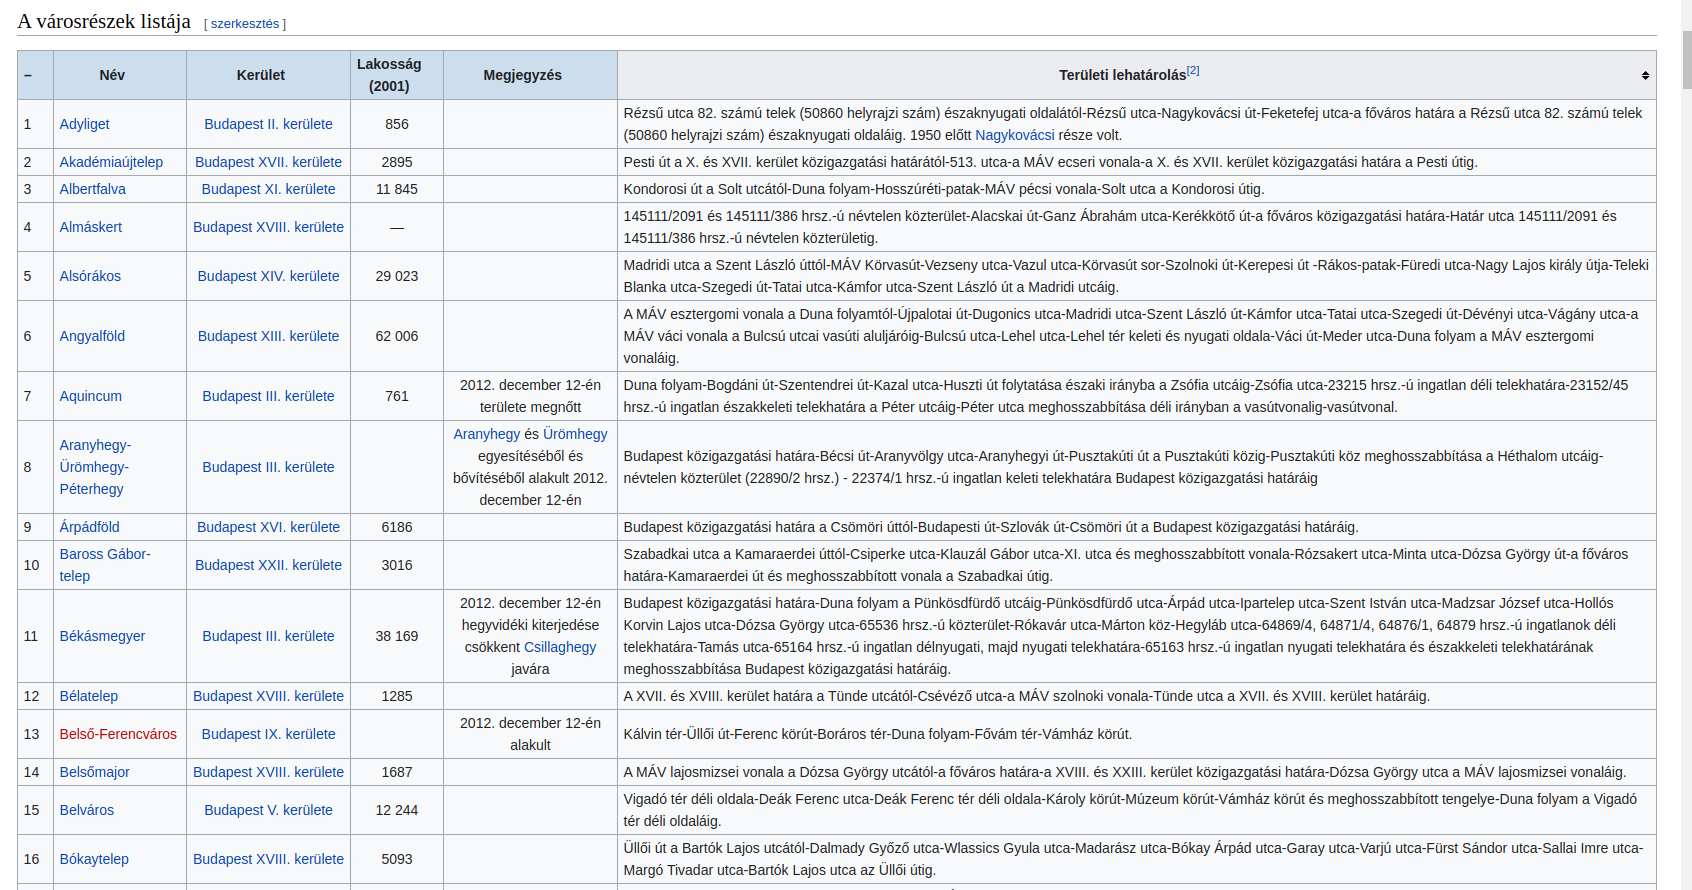
\includegraphics[width=1\linewidth]{neighbourhoods}
		\caption{Image about the table from Wikipedia}
		\label{fig:neighbourhoods}
	\end{figure}
	
	\item \url{https://api.foursquare.com}\\
	We use the \textit{Foursquare} API the explore the areas and retrieve the necessary information that correspond to the above problem description.
	\begin{figure}[!h]
		\centering
		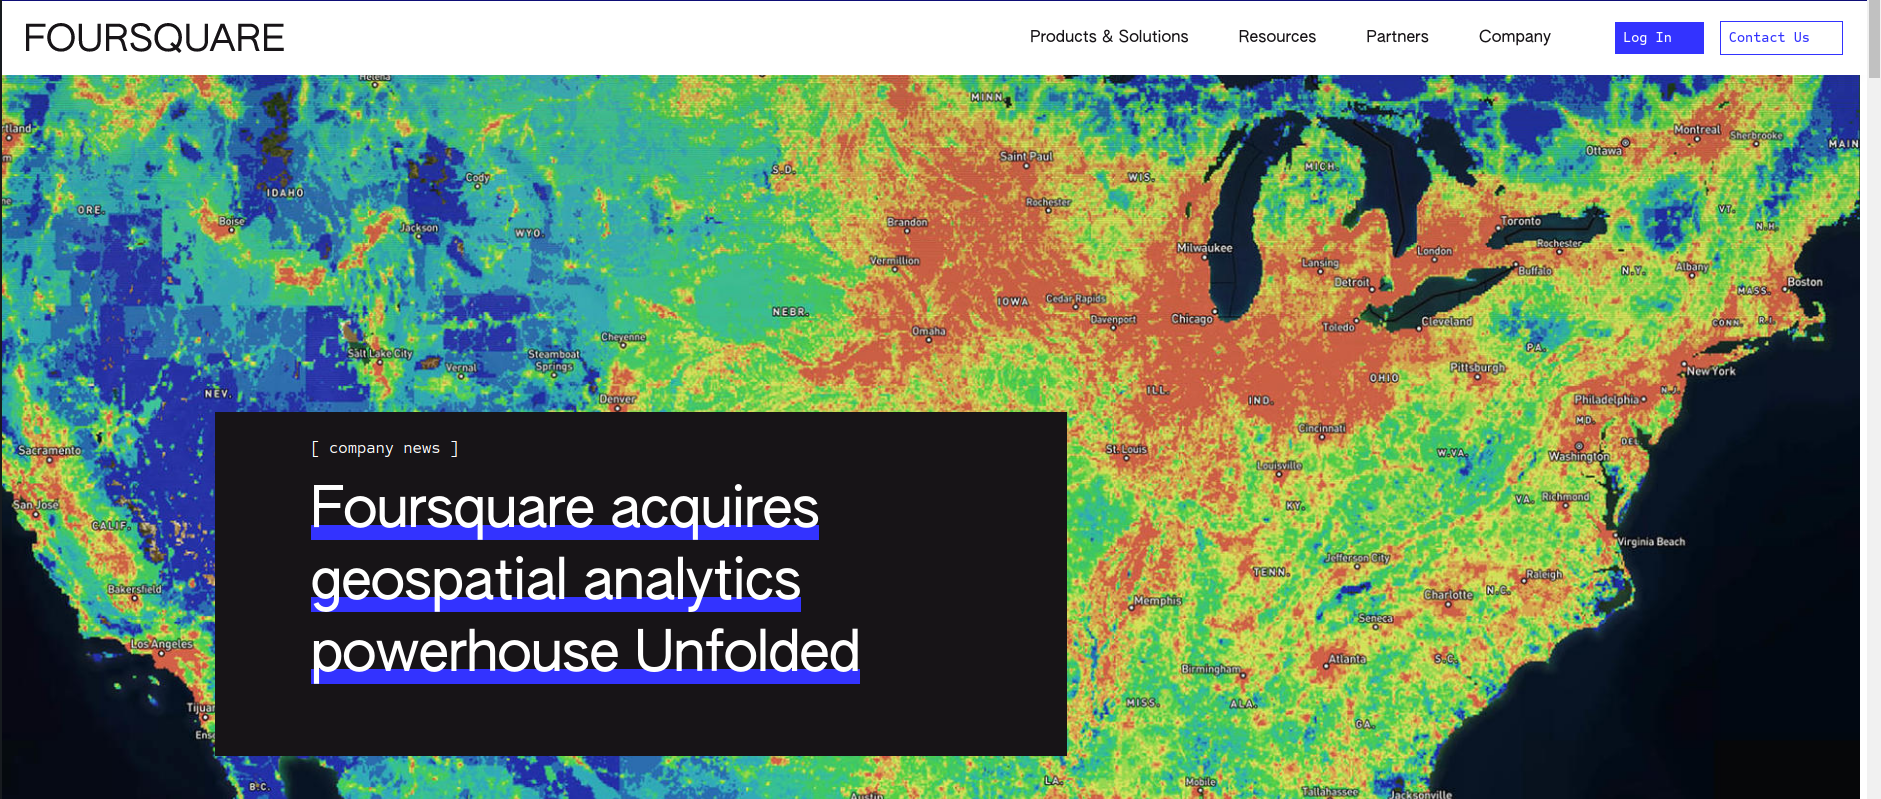
\includegraphics[width=1\linewidth]{foursquare}
		\caption{Homepage of the Foursquare application}
		\label{fig:foursquare}
	\end{figure}
	During the API calls, we filters for the mentioned categories of the venues: caf�s, universities and offices. Foursquare API has an option to restrict our exploration to several type of venues, see Figure~\ref{fig:categories}.
	\begin{figure}[!h]
		\centering
		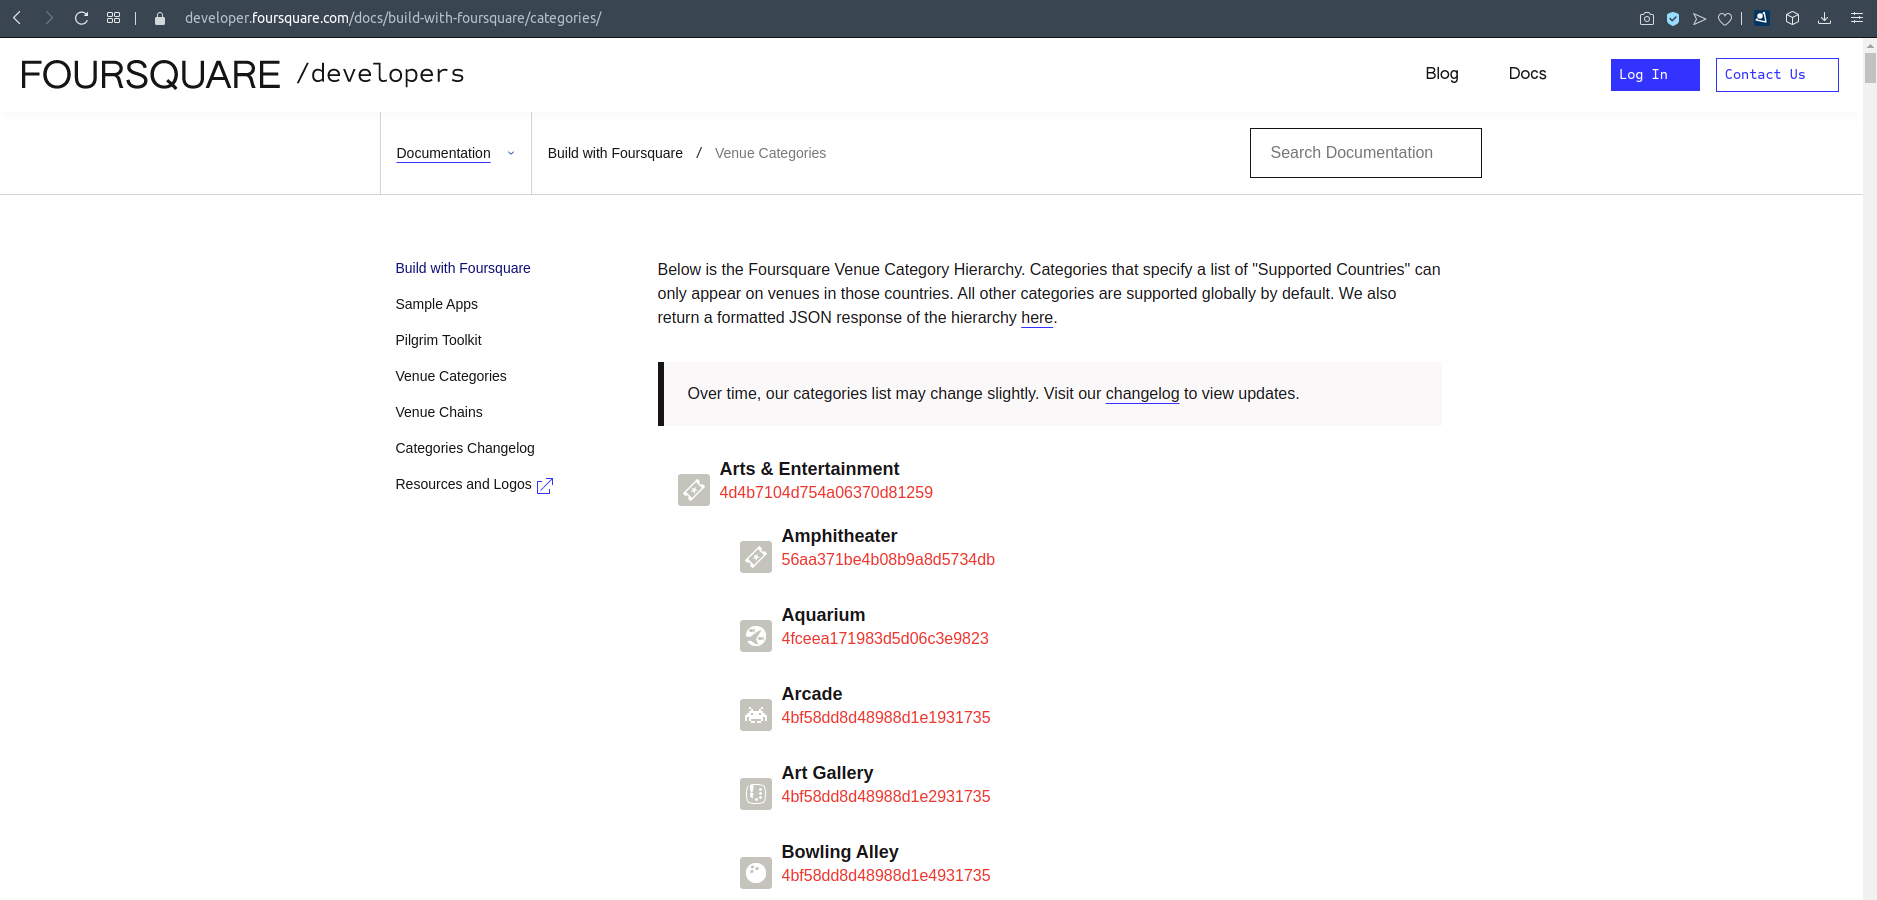
\includegraphics[width=1\linewidth]{foursquare2}
		\caption{List of available categories in Foursquare API}
		\label{fig:categories}
	\end{figure}
\end{enumerate}

To demonstrate this, I illustrate the data on the neighbourhood Gell�rthegy of the district I od Budapest. If we want to focus for the nearby office buildings, we make the API call
\begin{center}
	\url{https://api.foursquare.com/v2/venues/explore?&client_id=CLIENT_ID&client_secret=SECRET_CLIENT_ID&v=20180605&ll=47.492064,19.037200&radius=300&limit=100&categoryId=4bf58dd8d48988d124941735}
\end{center}
that retrieves with the following JSON data with 4 different venues from the office category.

\lstinputlisting[language=json]{sample.json}

\section*{Methodology}

The Wikipedia page will be scraped by a \textit{Python} library, that is \textit{Beautiful Soup}, to save the name of the districts, and neighbourhoods of Budapest into a \textit{pandas} \textit{dataframe}. Some data cleaning will be necessary, because in the original table there are some neighbourhoods that correspond to more than one districts, and we separate them by an easy string manipulation technique to get unique district-neighbourhood pairs.

Then, with another \textit{Python} client, \textit{GeoPy}, we locate the centres of neighbourhoods using \textit{Nominatim} and \textit{Photon} geocoding services.

After this point, we have the full list of neighbourhoods of Budapest, and we make several Foursquare API calls to retrieve the information about the number of caf�s, university buildings and office buildings.

We will cluster these informations as a three dimensional space to locate the similar neighbourhoods using k-means clustering algorithm.  After clustering, we can suggest a location where to rent an office to a new, small, but growing IT company.



\end{document}
